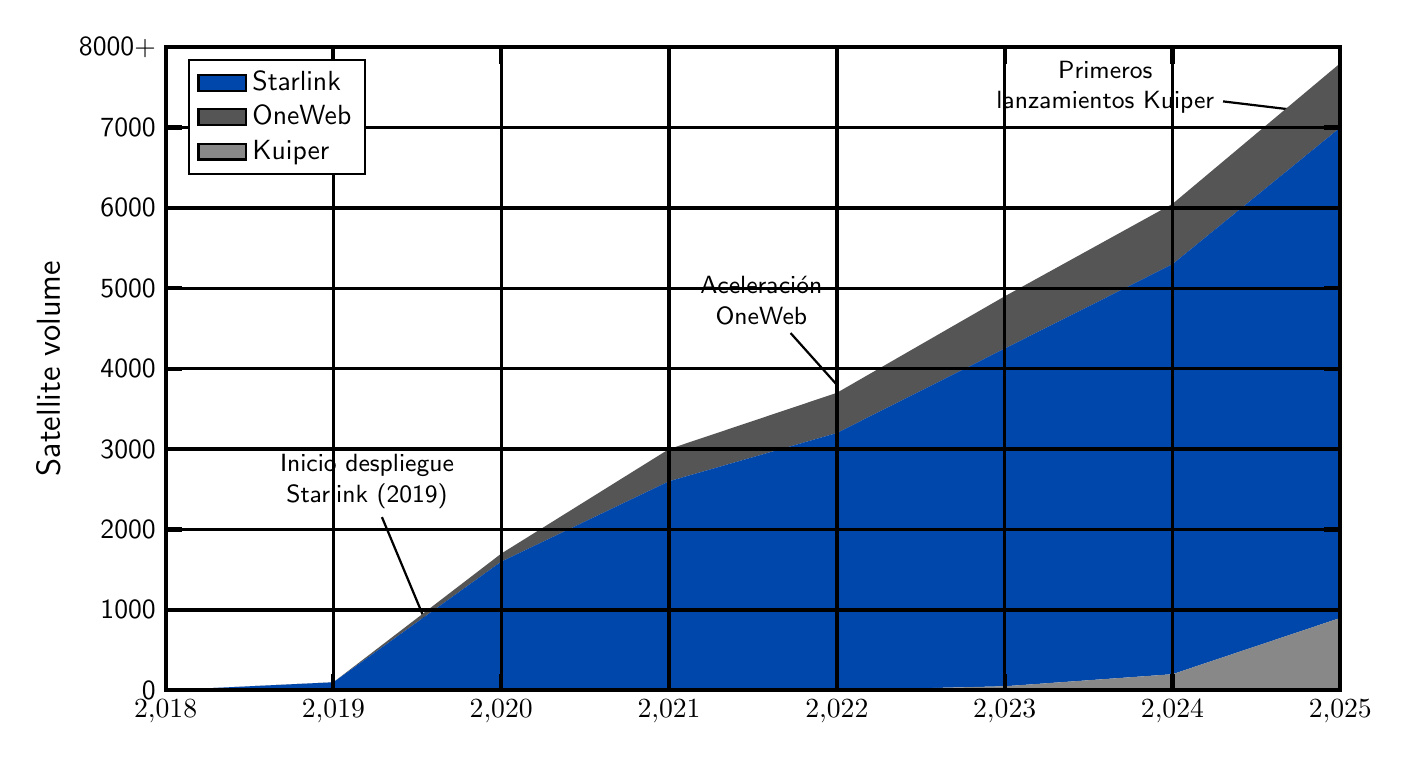
\begin{tikzpicture}

% === PARÁMETROS ===
% Colores
\definecolor{colorStarlink}{HTML}{0047AB}
\definecolor{colorOneWeb}{HTML}{555555}
\definecolor{colorKuiper}{HTML}{888888}
\definecolor{colorGrid}{HTML}{000000}
\definecolor{colorBg}{HTML}{FFFFFF}

% Dimensiones de la figura (Proporción 11 x 6.5 del figsize)
\def\figWidth{16.5cm}
\def\figHeight{9.75cm}

% Ejes y límites
\def\xmin{2018}
\def\xmax{2025}
\def\ymin{0}
\def\ymax{8000}

% Grosores de línea
\def\gridLineWidth{1.2pt}
\def\spineLineWidth{1.5pt}
\def\annoLineWidth{0.8pt}

% Coordenadas de anotación 1 (Starlink)
\def\annoOneXText{2019.2}
\def\annoOneYText{2600}
\def\annoOneXTarget{2019.6}
\def\annoOneYTarget{600}

% Coordenadas de anotación 2 (OneWeb)
\def\annoTwoXText{2021.55}
\def\annoTwoYText{4850}
\def\annoTwoXTarget{2022.0}
\def\annoTwoYTarget{3800}

% Coordenadas de anotación 3 (Kuiper)
% ASUNCIÓN: La flecha 3 se fuerza a apuntar a la capa gris oscura para ser fiel a la imagen generada (alucinación visual), 
% aunque lógicamente Kuiper sea la capa gris clara inferior.
\def\annoThreeXText{2023.6}
\def\annoThreeYText{7500}
\def\annoThreeXTarget{2024.8}
\def\annoThreeYTarget{7200}

% Estilos TikZ
\tikzset{
    annotation node/.style={
        align=center,
        font=\small\sffamily,
        inner sep=3pt
    },
    annotation link/.style={
        draw=black,
        line width=\annoLineWidth,
        solid
    }
}

% === ESTRUCTURA PRINCIPAL ===
\begin{axis}[
    width=\figWidth,
    height=\figHeight,
    axis background/.style={fill=colorBg},
    xmin=\xmin, xmax=\xmax,
    ymin=\ymin, ymax=\ymax,
    xtick={2018,2019,2020,2021,2022,2023,2024,2025},
    ytick={0,1000,2000,3000,4000,5000,6000,7000,8000},
    yticklabels={0, 1000, 2000, 3000, 4000, 5000, 6000, 7000, 8000+},
    ylabel={Satellite volume},
    ylabel style={font=\large\sffamily},
    tick label style={font=\normalsize\sffamily},
    % Estilo del recuadro
    axis line style={line width=\spineLineWidth, color=black},
    tick style={line width=\spineLineWidth, color=black},
    major tick length=6pt,
    % Grilla configurada para verse por encima de las capas
    xmajorgrids=true,
    ymajorgrids=true,
    grid style={color=colorGrid, line width=\gridLineWidth, solid},
    axis on top=true, % Equivalente a set_axisbelow(False)
    % Configuración del apilamiento
    stack plots=y,
    area style,
    enlarge x limits=false,
    % Configuración de leyenda
    legend style={
        at={(0.02, 0.98)},
        anchor=north west,
        font=\normalsize\sffamily,
        draw=black,
        line width=0.8pt,
        cells={anchor=west},
        fill=white,
        fill opacity=1,
        text opacity=1,
        outer sep=0pt
    }
]

% === ENTRADAS DE LEYENDA MANUALES ===
% Construcción manual de la leyenda para respetar el orden visual de Python
\addlegendimage{area legend, fill=colorStarlink, draw=black}
\addlegendentry{Starlink}
\addlegendimage{area legend, fill=colorOneWeb, draw=black}
\addlegendentry{OneWeb}
\addlegendimage{area legend, fill=colorKuiper, draw=black}
\addlegendentry{Kuiper}

% === DATOS ===
% Los "forget plot" evitan que estos comandos reescriban nuestra leyenda manual
% Capa 1: Kuiper (Base inferior)
\addplot[fill=colorKuiper, draw=none, forget plot] coordinates {
    (2018,0) (2019,0) (2020,0) (2021,0) (2022,0) (2023,50) (2024,200) (2025,900)
} \closedcycle;

% Capa 2: Starlink (Intermedia principal)
\addplot[fill=colorStarlink, draw=none, forget plot] coordinates {
    (2018,0) (2019,100) (2020,1600) (2021,2600) (2022,3200) (2023,4200) (2024,5100) (2025,6100)
} \closedcycle;

% Capa 3: OneWeb (Superior)
\addplot[fill=colorOneWeb, draw=none, forget plot] coordinates {
    (2018,0) (2019,0) (2020,100) (2021,400) (2022,500) (2023,650) (2024,750) (2025,800)
} \closedcycle;

% === ANOTACIONES ===
% Anotación 1: Starlink
\node[annotation node] at (axis cs:\annoOneXText,\annoOneYText) {Inicio despliegue\\Starlink (2019)}
    edge[annotation link] (axis cs:\annoOneXTarget,\annoOneYTarget);

% Anotación 2: OneWeb
\node[annotation node] at (axis cs:\annoTwoXText,\annoTwoYText) {Aceleración\\OneWeb}
    edge[annotation link] (axis cs:\annoTwoXTarget,\annoTwoYTarget);

% Anotación 3: Kuiper
\node[annotation node] at (axis cs:\annoThreeXText,\annoThreeYText) {Primeros\\lanzamientos Kuiper}
    edge[annotation link] (axis cs:\annoThreeXTarget,\annoThreeYTarget);
    
\end{axis}
\end{tikzpicture}